\documentclass[UTF8]{article}
\usepackage{tikz}
\usetikzlibrary{calc,intersections,through}
\usepackage{ctex}
\usepackage{multirow,makecell}
\usepackage{booktabs}

\begin{document}
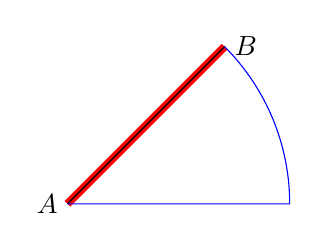
\begin{tikzpicture}

    \coordinate [label=left:$A$] (A) at (0,0);
    \coordinate [label=right:$B$] (B) at (2,2);

    \draw[red,line width=1mm] let \p1=($(B)-(A)$) in (A) --++ (45:({veclen(\x1,\y1)}););
    \draw (A) -- (B);
    \draw[blue] (A) let \p1 = ($(B)-(A)$) in --++({veclen(\x1,\y1)},0) arc (0:45:({veclen(\x1,\y1)}););

\end{tikzpicture}

\begin{table}
    \centering
    \begin{tabular}{|c|c|c|c|}
        \hline
        \multirow{2}{*}{$r$} & \multicolumn{2}{c|}{\footnotesize{圆心坐标}} & \multirow{2}{*}{\footnotesize{半径} $\left(\frac{1}{1+r}\right)$}       \\
        \cline{2-3}
                             & $\Gamma_r=\frac{r}{1+r}$                 & $\Gamma_i=0$       &       \\
        \hline
        0                    & 0                                        & 0                  & 1   \\
        \hline
        1                    & 1/2                                      & 0                  & 1/2 \\
        \hline
        2                    & 2/3                                      & 0                  & 1/3 \\
        \hline
    \end{tabular}
    \caption{A test caption}
    \label{table1}
\end{table}

\begin{tabular}{|c|c|c|c|c|}
    \hline
    \multirow{2}{*}{Multi-Row}        &  \multicolumn{2}{c|}{Multi-Column}  &  \multicolumn{2}{c|}{\multirow{2}{*}{Multi-RowandCol}}   \\
    \cline{2-3}
                                      & column-1 & column-2 & \multicolumn{2}{c|}{}           \\
    \hline
    label-1                           & label-2  & label-3  & label-4               & label-5 \\
    \hline
\end{tabular}

\begin{tabular}{|c|c|}
    \hline
    \textbf{阻抗圆图} & \textbf{导纳圆图} \\ \hline
    $r$           & $g$           \\ \hline
    $x$           & $b$           \\ \hline
    $\Gamma(z)$   & $\Gamma_I(z)$ \\ \hline
    电压振幅值腹点       & 电流振幅值腹点       \\ \hline
    电压振幅值节点       & 电流振幅值节点       \\ \hline
    开路点           & 短路点           \\ \hline
    短路点           & 开路点           \\
    \hline
\end{tabular}

\end{document}